\documentclass[eng,openany]{mgr}
\usepackage{listings}
\usepackage[english]{babel}
\usepackage{graphicx}
\usepackage{hyperref}
\usepackage{tabularx,colortbl} 
\usepackage{rotating}
\usepackage[utf8]{inputenc} 
\setlength\parindent{24pt}

%tlmgr init-usertree
%sudo apt-get install xzdec
%sudo tlmgr install collection-fontsrecommended



% Default fixed font does not support bold face
\DeclareFixedFont{\ttb}{T1}{txtt}{bx}{n}{12} % for bold
\DeclareFixedFont{\ttm}{T1}{txtt}{m}{n}{12}  % for normal

% Custom colors
\usepackage{color}
\definecolor{deepblue}{rgb}{0,0,0.5}
\definecolor{deepred}{rgb}{0.6,0,0}
\definecolor{deepgreen}{rgb}{0,0.5,0}

\usepackage{listings}

% Python style for highlighting
\newcommand\pythonstyle{\lstset{
language=Python,
basicstyle=\ttm,
otherkeywords={self},             % Add keywords here
keywordstyle=\ttb\color{deepblue},
emph={MyClass,__init__},          % Custom highlighting
emphstyle=\ttb\color{deepred},    % Custom highlighting style
stringstyle=\color{deepgreen},
frame=tb,                         % Any extra options here
showstringspaces=false            % 
}}


% Python environment
\lstnewenvironment{python}[1][]
{
\pythonstyle
\lstset{#1}
}
{}

% Python for external files
\newcommand\pythonexternal[2][]{{
\pythonstyle
\lstinputlisting[#1]{#2}}}

% Python for inline
\newcommand\pythoninline[1]{{\pythonstyle\lstinline!#1!}}


\renewcommand\lstlistlistingname{List of code listings}
\newcommand{\linia}{\rule{\linewidth}{0.4mm}}
\author{Jarosław Szumega\\Ilona Brzozowska}
\title{Histogram equalization algorithm implementation.}
\engtitle{}
\supervisor{Marek Woda, Ph.D.}
\field{Computer Science}
\specialisation{Internet Enginering}
\date{10.01.2016}
\begin{document}
\maketitle
\tableofcontents
\chapter{Project description}
\section{Subject}
The main goal of following project is to choose and to implement an algorithm that will perform histogram equalization.\\
Such an operation is required e.g. when photo/picture was over- or underexposed by light. As a result it is too bright or too dark to be properly percept by human eye.
\begin{figure}[h]
\centering
\includegraphics[width=0.7\linewidth]{./lena-histogram}
\caption{'Lena image' - before and after equalizer applied.}
\label{fig:lena-histogram}
\end{figure}

\section{Scope}
The work may be divided into parts:
\begin{itemize}
\item research related to image processing and histogram normalization,
\item implementation selected algorithm and all necessary tools,
\item quality comparison.
\end{itemize}

The result should be useful tool to perform image improvements - histogram equalization - at a level that in fact will improv image general look.
\\
\\
When working solution will be present, th simple tests with built-in Octave/Matlab functions will be performed.

\section{Chosen technologies}
During project classes, the following technologies had been agreed with supervisor:
\begin{itemize}
\item Unix systems,
\item using Octave engine for image processing,
\item Python as programming environment,
\item PyQt for user-friendly GUI.
\end{itemize}
The result will be simple program that wraps essential functions into graphical interface - just to simplify usage of histogram correction.
\chapter{Implementation}
\section{Performance issues}
The essential part of project are own-written Octave scripts, that perform image processing. As it turned out during developing matrix operations - it is much faster than using Python-defined algorithms.\\
To achieved cooperation between python interpreter and Octave (native and own functions) there was used \textbf{oct2py} module.
It simply allows to set up octave session, configure it and call either built-in functions or defined by user.\\
After that they can be called as a engine object methods.
\\
\\
\textbf{Listing 2.1 Using octave engine.}
\begin{python}
        octave = oct2py.Oct2Py()
        octave.addpath('./scripts')
        octave.pkg('load', 'image')
\end{python}
\section{Functions in Octave}
The most essential function is the one that combines performing equalization with proper pre- and postprocessing. The image type shall be detected. It is necessary because:
\begin{itemize}
\item grayscale images need histogram equalization just to be applied on matrix that represents them,
\item RGB images at first should be convert to YUV. Then on Y-part the qualization is performed. YUV is agai combained togther and converted into RGB.
\end{itemize}

As it was stated before -  the project consist also of user-defined methods written specifically for image processing.The following functions are own work of author:
\begin{itemize}
\item higher-level histogram performer,
\item histogram equalization algorithm (uniform),
\item converter between RGB and YUV (both directions),
\end{itemize}
\newpage
\noindent
\textbf{Listing 2.2 Histogram correction with post- and preprocessing}
\begin{python}
function img = hist_processings(I)
[rows,columns,channels] =  size(I);

if channels == 1
  img = histcor(I);

else
  yuv = rgb2yuv(I);
  ui = yuv(:,:,1);
  ui = ui.*255;
  ui = uint8(ui);
  ui = histcor(ui);
  yuv(:,:,1) = double(ui)./255;
  img = yuv2rgb(yuv);
end
imwrite(img,'tmp.png');
end
\end{python}
\vspace{30pt}
\textbf{Listing 2.3 Histogram equalization algorithm}\\
(stretching histogram in 'uniform' way)
\begin{python}
function cor = histcor(img)

for i=1:256
h(i) = sum(sum(img==i-1));
end

cor = img;
s = sum(h);

for i = 1:256
I = find(img==i-1);
cor(I) = sum(h(1:i))/s*255;
end
\end{python}
\newpage
\section{GUI in Python}
Really important part is designing user interface. It should be simple, but also designed with care to be practical.
\\
\\
Qt Designer was used to prepare window and its controls in drag'n'drop way \ref{fig:qtdesigner}.
\begin{figure}[h]
\centering
\includegraphics[width=0.7\linewidth]{./qtdesigner}
\caption{QtDesigner tool for designing user interface.}
\label{fig:qtdesigner}
\end{figure}

After creation of *.ui file, the intrface can be converted to a form that allow to use it from Python (import as a module).
\begin{python}
\$ pyuic4 hist.ui > hist_gui.py
\end{python}
\noindent
That creates Python code responisble for Qt window and element drawing. But still, the functionality does not exist!\\
\\
To connect gui events with python code, the signal/slot \ref{fig:signals} mechanism was applied.
\begin{figure}[h]
\centering
\includegraphics[width=0.4\linewidth]{./signals}
\caption[h]{}
\caption{Illustration of signal/slot mechanism.}
\label{fig:signals}
\end{figure}
\newpage\noindent
Defining connection between signal and slot can be done in following way:
\\
\\
\textbf{Listing 2.4 Adding action for buttons click event.}
\begin{python}
        self.ui.loadButton.clicked.connect(self.openFile)
        self.ui.showButton.clicked.connect(self.imShow)
        self.ui.eqButton.clicked.connect(self.equalize)
        self.ui.cmpButton.clicked.connect(self.compare)
\end{python}
\vspace{30pt}
\textbf{Fixing issues}\\
One last remark is about cooperation between Octave engine and Python. Not always the entire data was properly transfered between engine and interpreter (especially in case of multidimensional arrays like in RGB images).\\
To solve it, the solution from graphics editors was mimicked - the engine saves \textit{temporary file} to be read by Python-based program.

\chapter{Results}
\section{System at work}
A few images was tested to evaluat if th program works correctly.
The result are really promising (pictures \ref{fig:color}, \ref{fig:park}). Especially taking dark, grayscale images.
\begin{figure}[h]
\centering
\includegraphics[width=0.7\linewidth]{./color}
\caption{RGB image with slightly underexposure.}
\label{fig:color}
\end{figure}
\begin{figure}[h]
\centering
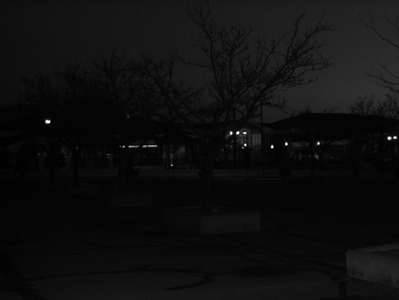
\includegraphics[width=0.7\linewidth]{./park}
\caption{Photo taken by night - almost impossible to catch details.}
\label{fig:park}
\end{figure}
\newpage
\section{Comparison to native functions}
To compare own histogram correction with Octave's \textbf{histeq()} function, the proper script was prepared.

In every case, the Octave algorithm is much faster than hand-written one. But during testing there was an example where author's implementation is better:
\begin{figure}[h]
\centering
\includegraphics[width=0.7\linewidth]{./cmp}
\caption{Native function confronts user-defined.}
\label{fig:cmp}
\end{figure}
As it can be seen with naked eye -the Octave native produces some kind of artifacts. The transition between pixels is not smooth.\\
\\
In case of author function - there is no such a problem. The image is definitely more 'readable' and it is with no disturbing artifacts.
\section{Summary}
The histogram equalization may help not only fixing not well exposured files, but also to see the previously not seen details (like in case of night scenario).
\\
\\
The intersting issue is also fact, that user-defined algorithm can beat specialist's work and perform better visual effect. Although in case of time execution, the native solution is a lot faster.
\begin{figure}[h]
\centering
\includegraphics[width=0.3\linewidth]{./img}
\caption{Values are in order Octave time, author's time.}
\label{fig:img}
\end{figure}

\end{document}
